\section{Direzioni di Ricerca Future}

\subsection{Strumenti per Query Rewriting}
\begin{frame}{Strumenti per Query Rewriting}
    \begin{block}{Problema}
        Utilizzare ontologie mai viste potrebbe essere difficoltoso, soprattutto per la mancanza di confidenza con il vocabolario usato.
    \end{block}
    
    \begin{example}
        Un ontologia rappresenta una caserma ove son presenti Cani polizziotto, rappresentati dal nome CanePol. L'idea sarebbe che l'user nella query usa solamente "cane", e il sistema riscrive la query con "CanePol".    
    \end{example}
\end{frame}
\begin{frame}
    \begin{block}{Idea di soluzione}
        La nostra proposta consiste nel creare uno strumento per riscrivere le query, utilizzando una combinazione di strumenti come 
        \begin{itemize}
            \item tecnologie per l'analisi del linguaggio naturale
            \item un sistema di tipi statico che controlla la correttezza della query riscritta 
        \end{itemize}
    \end{block}

    \begin{block}{Direzione pratica di ricerca}
        Una direzione pratica potrebbe essere usare reti di parole come Babelnet\footnotemark ~ per sostituire il vocabolo "cane" con quello semanticamente più vicino nell'ontologia, ovvero "CanePol".
    \end{block}
    \footnotetext{https://babelnet.org/}
\end{frame}



\subsection{Tipi per RDF/XML con CDuce}
\begin{frame}{Tipi per RDF/XML con CDuce}
    \begin{block}{CDuce}
        CDuce\footnotemark ~ è un linguaggio funzionale tipato che permette di produrre XML corretto a partire da specifiche formali (tipi) e viceversa. L'idea è utilizzare questo linguaggio per lavorare sui tipi anzichè direttamente sulle ontologie espresse in XML, in modo da facilitare il lavoro.
    \end{block}
    \footnotetext{https://www.cduce.org/}
\end{frame}

\begin{frame}{Merging di ontologie}
    \begin{itemize}
        \item Il problema del merging di ontologie, che consiste nell'unire due ontologie, può essere ridotto al problema del merging tra due tipi usando CDuce:
    \end{itemize}
    
    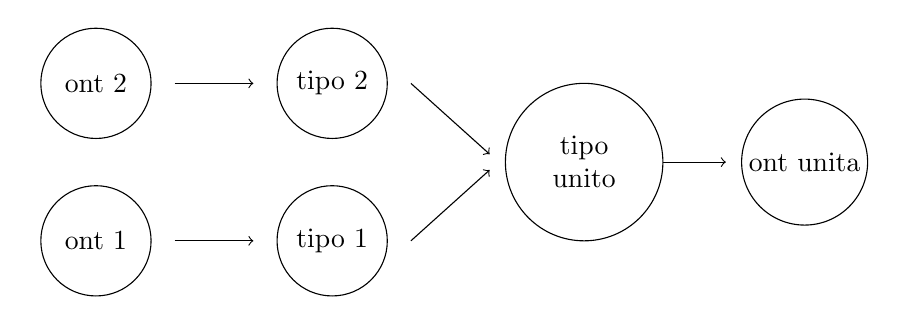
\begin{tikzpicture}
        \draw (0,0) circle (0.7cm);
        \draw (0,2) circle (0.7cm);
        \draw [->] (1,0) -- (2,0);
        \draw [->] (1, 2) -- (2,2);
        \draw (3,0) circle (0.7cm);
        \draw (3,2) circle (0.7cm);
        \draw [->] (4,0) -- (5, 0.9);
        \draw [->] (4,2) -- (5, 1.1);
        \draw (6.2, 1) circle (1cm);
        \draw [->] (7.2, 1) -- (8, 1);
        \draw (9, 1) circle (0.8cm);
        \node[text width=1.5cm, align=center] at (0,0) {ont 1};
        \node[text width=1.5cm, align=center] at (0,2) {ont 2};
        \node[text width=1.5cm, align=center] at (3,0) {tipo 1};
        \node[text width=1.5cm, align=center] at (3,2) {tipo 2};
        \node[text width=1.5cm, align=center] at (6.2, 1) {tipo unito};
        \node[text width=1.5cm, align=center] at (9,1) {ont unita};
    \end{tikzpicture}
        
\end{frame}

\subsection{Tipi per FRBR}
\begin{frame}{Tipi per FRBR}
    \begin{block}{FRBR}
    Per Functional Requirements for Bibliographic Records (FRBR) si intende uno
    schema concettuale sviluppato dalla International Federation of Library Associations
    and Institutions (IFLA), realizzato tramite modello entità-relazione allo scopo di dare
    una rappresentazione semi-formale alle informazioni bibliografiche.
    \end{block}
    ~\\
    FRBR descrive:
    \begin{itemize}
        \item Le \blue{opere}
        \item Le \blue{organizzazioni} che sono responsabili delle opere
        \item I \blue{soggetti} delle opere
    \end{itemize}
\end{frame}

\begin{frame}{Tipi per FRBR}
Le opere sono classificate secondo i livelli:
\begin{itemize}
    \item \blue{work} (opera)
    \item \blue{expression} (espressione)
    \item \blue{manifestation} (manifestazione)
    \item \blue{item} (oggetto concreto)
\end{itemize}
\begin{example}
\begin{itemize}
    \item \blue{Work}: The Last of Us Part I (VideoGame), The Last of Us (Serie TV).
    \item \blue{Expression}: The Last of Us Part I traduzione italiana e versione orginale.
    \item \blue{Manifestation}: The Last Of Us versione Disco e versione digitale.
    \item \blue{Item}: Copia fisica (o digitale) di The Last of Us.
\end{itemize}
\end{example}
\end{frame}

\begin{frame}{Tipi per FRBR}
	Punto di partenza:
	\begin{center}
		\blue{Work come \textit{tipo}} (perchè astratto)
	\end{center}
    Due possibili ambiti:
    \begin{itemize}
     \item \blue{Retrieving} di duplicati di un'opera.\hfill{\color{green} obiettivo facile}
     \begin{example}
     	I due work registrati come "dark (TV)" e "Dark (TV)" sono duplicati.
     \end{example}
     \item \blue{Ristrutturazione} di biblioteche virtuali.\hfill{\color{magenta} obiettivo ambizioso}\\
     $\implies$ Usare i tipi per convertire in formato FRBR dati non strutturati.
    \end{itemize}
    Problemi aperti:
    \begin{itemize}
        \item \`e davvero \blue{work} il punto di partenza?
        \item esplorare i vari supporti necessari:
        \begin{itemize}
        	\item analisi sintattica
        	\item analisi del linguaggio naturale.
        \end{itemize}
    \end{itemize}
\end{frame}

\subsection{Tipi per Costruire e Ristrutturare Ontologie}

\begin{frame}{Tipi per Costruire e Ristrutturare Ontologie}
	\begin{itemize}
		\item Nei processi di creazione di un’ontologia, la tendenza attuale è di riutilizzare il più possibile le ontologie invece che crearle da zero. 
	
		\item \blue{NeOn}\footnote{\url{http://neon-project.org/}} è stata una delle prime metodologie per sviluppare un'ontologia, sfruttando specialmente il riutilizzo delle risorse di conoscenza disponibili.
	\end{itemize}
	\begin{block}{Riutilizzo di un'ontologia}
		Il processo in cui la conoscenza ontologica esistente viene utilizzata come input per generare nuove ontologie.
	\end{block}
	
\end{frame}

\begin{frame}{Tipi per Costruire e Ristrutturare Ontologie}
	NeOn definisce il riutilizzo di un'ontologia attraverso le attività di
\begin{enumerate}
	\item \blue{ricerca},
	\item \blue{valutazione},
	\item \blue{comparazione} e
	\item \blue{integrazione} delle ontologie esistenti.
\end{enumerate}
Queste operazioni sono spesso soggette a errori dati da incoerenze o eterogeneità fra le informazioni presenti nelle sorgenti di conoscenza.\\~\\
$\implies$ Il processo di riutilizzo di un'ontologia diventa \blue{dispendioso in termini di tempo} per lo sviluppatore, di cui non è possibile rimuovere il contributo dal processo creativo.
\end{frame}

\begin{frame}{Tipi per Costruire e Ristrutturare Ontologie}
	 \begin{block}{La nostra idea}
	 	Fornire allo sviluppatore degli strumenti formali basati su linguaggi funzionali tipati statisticamente da utilizzare per aiutarlo nel capire se il suo processo stia effettivamente producendo il risultato desiderato e/o suggerire cambiamenti.
	 \end{block}
	 Attualmente esistono già degli strumenti più o meno formali per agevolare questo processo, es. \textsc{\blue{PROMPT}} in Prot\'eg\'e, \textsc{\blue{FCA-Merge}}, etc.
	 \begin{example}
	 	La proprietà di composizionalità applicata alle ontologie potrebbe automatizzare la modularizzazione, per considerare solo la parte rilevante per il processo in atto.
	 \end{example}
\end{frame}

\section{I nostri contributi}
\begin{frame}{I nostri contributi}
    \begin{itemize}
        \item Studio di una parte dello \blue{stato dell'arte} sull'applicazione dei linguaggi funzionali e dei tipi per il Web Semantico.\\~\\
        \item Studio e \blue{implementazione del $\lambda_{DL}$} e in particolare la correttezza e l'abitabilità delle query SPARQL.\\~\\
        \item Insieme alla consulenza scientifica di Marco Antonio Stranisci, Rossana Damiano e Antonio Lieto abbiamo speculato una serie di \blue{possibili direzioni future}:
            \begin{itemize}
                \item Tipi per Query Rewriting
                \item Tipi per RDF/XML con CDuce
                \item Tipi per FRBR
                \item Tipi per costruire e ristrutturare ontologie
            \end{itemize}
    \end{itemize}
\end{frame}